\documentclass[12pt]{article}
\usepackage{times} 			% use Times New Roman font

\usepackage[margin=1in]{geometry}   % sets 1 inch margins on all sides
\usepackage[hidelinks]{hyperref}               % for URL formatting
\usepackage[pdftex]{graphicx}       % So includegraphics will work
\setlength{\parskip}{1em}           % skip 1em between paragraphs
\usepackage{indentfirst}            % indent the first line of each paragraph
\usepackage{datetime}
\usepackage[small, bf]{caption}
\usepackage{listings}               % for code listings
\usepackage{xcolor}                 % for styling code
\usepackage{multirow}
\usepackage{adjustbox}
\usepackage{caption}


%New colors defined below
\definecolor{backcolour}{RGB}{246, 246, 246}   % 0xF6, 0xF6, 0xF6
\definecolor{codegreen}{RGB}{16, 124, 2}       % 0x10, 0x7C, 0x02
\definecolor{codepurple}{RGB}{170, 0, 217}     % 0xAA, 0x00, 0xD9
\definecolor{codered}{RGB}{154, 0, 18}         % 0x9A, 0x00, 0x12

%Code listing style named "gcolabstyle" - matches Google Colab
\lstdefinestyle{gcolabstyle}{
  basicstyle=\ttfamily\small,
  backgroundcolor=\color{backcolour},   
  commentstyle=\itshape\color{codegreen},
  keywordstyle=\color{codepurple},
  stringstyle=\color{codered},
  numberstyle=\ttfamily\footnotesize\color{darkgray}, 
  breakatwhitespace=false,         
  breaklines=true,                 
  captionpos=b,                    
  keepspaces=true,                 
  numbers=left,                    
  numbersep=5pt,                  
  showspaces=false,                
  showstringspaces=false,
  showtabs=false,                  
  tabsize=2
}

\lstset{style=gcolabstyle}      %set gcolabstyle code listing

% to make long URIs break nicely
\makeatletter
\g@addto@macro{\UrlBreaks}{\UrlOrds}
\makeatother

% for fancy page headings
\usepackage{fancyhdr}
\setlength{\headheight}{13.6pt} % to remove fancyhdr warning
\pagestyle{fancy}
\fancyhf{}
\rhead{\small \thepage}
\lhead{\small HW\#5, Huang}  % EDIT THIS, REPLACE # with HW number
\chead{\small DATA 440, Fall 2022} 

%-------------------------------------------------------------------------
\begin{document}

% EDIT THE ITEMS HERE
\begin{centering}
{\large\textbf{Graph Partitioning}}\\ 
Sofia Huang\\
due 11/15/2022\\
\end{centering}

%-------------------------------------------------------------------------

% The * after \section just says to not number the sections
\section*{1. Color nodes based on final split}
\noindent \textbf{Draw the original Karate club graph (before the split) and color the nodes according to the factions they belong to (John A or Mr. Hi). This should look similar to the graph on slide 92 - all edges should be present, just indicate the nodes in the eventual split by color.}

\begin{figure}[h]
    \centering
    % trim and clip are used to crop the image, trim=left bottom right top
    % width sets max width, height will be scaled appropriately
    %\includegraphics[trim=0 20 10 50, clip, width=\textwidth]
    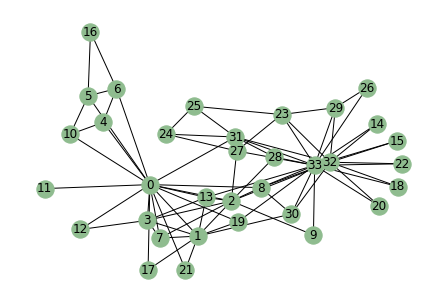
\includegraphics[width=300, scale=0.75]
    {KC_original.png}
    \caption{Original Karate Club graph.}
    \label{fig:original_kc}
\end{figure}

\begin{figure}[h]
    \centering
    % trim and clip are used to crop the image, trim=left bottom right top
    % width sets max width, height will be scaled appropriately
    %\includegraphics[trim=0 20 10 50, clip, width=\textwidth]
    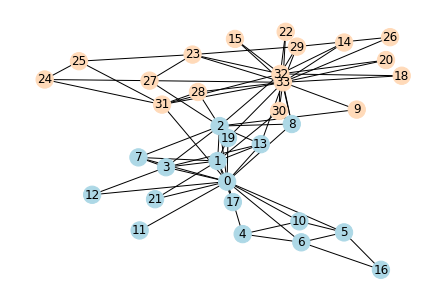
\includegraphics[width=300, scale=0.75]
    {KC_clubs.png}
    \caption{Split Karate Club graph.}
    \label{fig:split_kc}
\end{figure}

\clearpage

\noindent\textbf{Q: How many nodes (students) eventually go with John and how many with Mr. Hi?}

17 students eventually go with John and 17 go with Mr. Hi.\\

To draw the graphs, I used the python package Networkx and its built-in Karate Club graph function. Then, to color the nodes to represent the split, I created a dictionary that connected the club to the color I wanted those nodes to be. Then, I used list comprehension to create a list of colors that corresponds to the list of Karate Club graph nodes. Lastly, I drew the graph showing the split using the list of colors. The orange represents those who went with John and the blue represents the students who went with Mr Hi.

\begin{lstlisting}[language=Python, caption=Drawing the split Karate Club graph, label=lst:copy]
import networkx as nx
import matplotlib.pyplot as plt
K = nx.karate_club_graph()
club_color = {
    'Mr. Hi': 'lightblue',
    'Officer': 'peachpuff',
}
node_colors = [club_color[K.nodes[n]['club']] for n in K.nodes]
nx.draw(K, node_color=node_colors, with_labels=True)
\end{lstlisting}

\section*{2. Use the Girvan-Newman algorithm to illustrate the split}
\noindent \textbf{We know the final result of the Karate Club split, which you've colored in Q1. Use the Girvan-Newman algorithm to check if the split could have been predicted by the social interactions expressed by edges. How well does the mathematical model represent reality? Generously document your answer with all supporting equations, code, graphs, arguments, etc.\\Keeping the node colors the same as they were in Q1, run multiple iterations of the Girvan-Newman graph partioning algorithm (see Module-07 Social Networks, slides 90-99) on the Karate Club graph until the graph splits into two connected components. Include an image of the graph after each iteration in your report.}

\begin{figure}
\centering
\begin{minipage}{.5\textwidth}
  \centering
  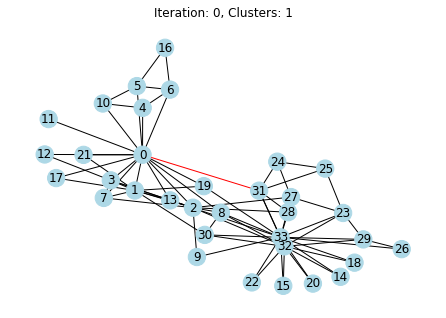
\includegraphics[width=250]{KC_GN0.png}
  \label{fig:GN0}
\end{minipage}%
\begin{minipage}{.5\textwidth}
  \centering
  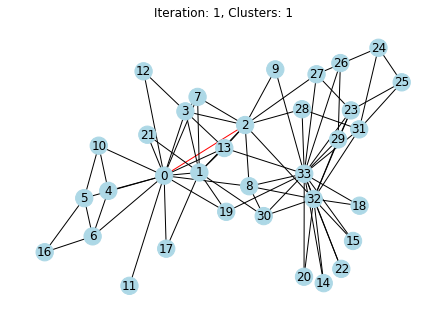
\includegraphics[width=250]{KC_GN1.png}
  \label{fig:GN1}
\end{minipage}
\end{figure}

\begin{figure}
\centering
\begin{minipage}{.5\textwidth}
  \centering
  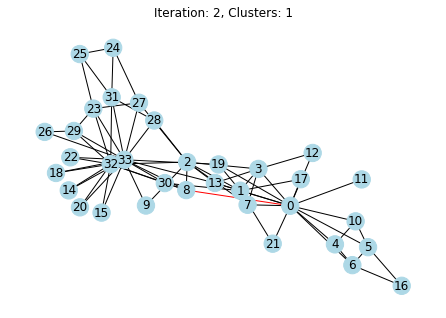
\includegraphics[width=250]{KC_GN2.png}
  \label{fig:GN2}
\end{minipage}%
\begin{minipage}{.5\textwidth}
  \centering
  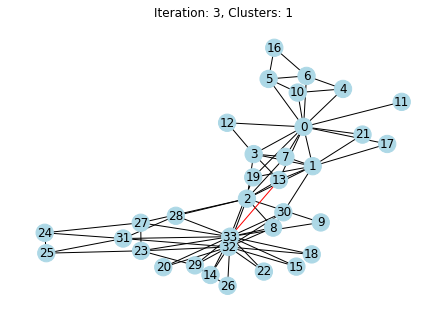
\includegraphics[width=250]{KC_GN3.png}
  \label{fig:GN3}
\end{minipage}
\end{figure}

\begin{figure}
\centering
\begin{minipage}{.5\textwidth}
  \centering
  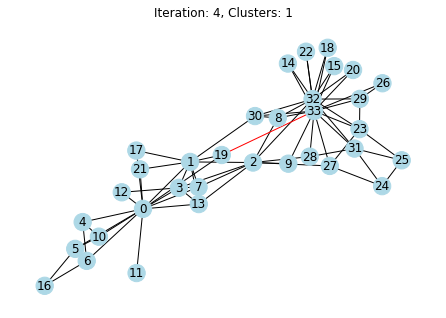
\includegraphics[width=250]{KC_GN4.png}
  \label{fig:GN4}
\end{minipage}%
\begin{minipage}{.5\textwidth}
  \centering
  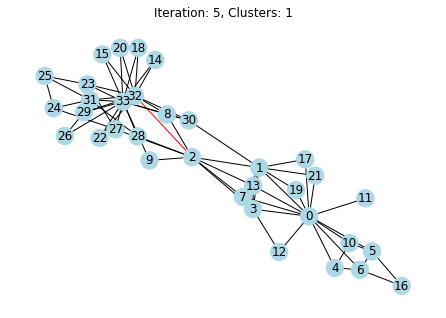
\includegraphics[width=250]{KC_GN5.png}
  \label{fig:GN5}
\end{minipage}
\end{figure}

\clearpage

\begin{figure}
\centering
\begin{minipage}{.5\textwidth}
  \centering
  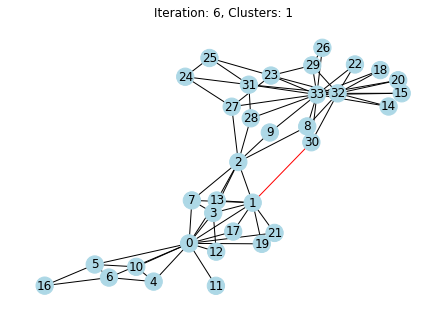
\includegraphics[width=250]{KC_GN6.png}
  \label{fig:GN6}
\end{minipage}%
\begin{minipage}{.5\textwidth}
  \centering
  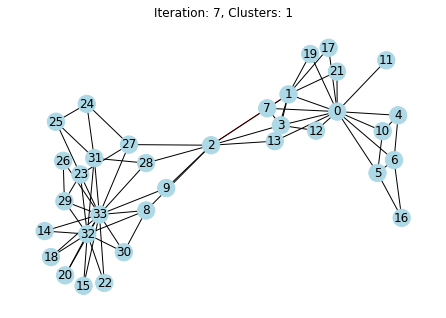
\includegraphics[width=250]{KC_GN7.png}
  \label{fig:GN7}
\end{minipage}
\end{figure}

\begin{figure}
\centering
\begin{minipage}{.5\textwidth}
  \centering
  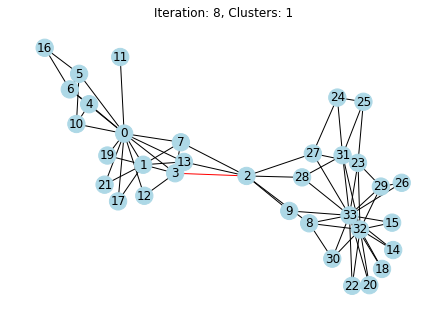
\includegraphics[width=250]{KC_GN8.png}
  \label{fig:GN8}
\end{minipage}%
\begin{minipage}{.5\textwidth}
  \centering
  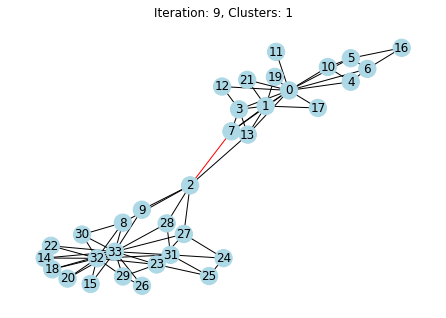
\includegraphics[width=250]{KC_GN9.png}
  \label{fig:GN9}
\end{minipage}
\end{figure}

\begin{figure}
\centering
\begin{minipage}{.5\textwidth}
  \centering
  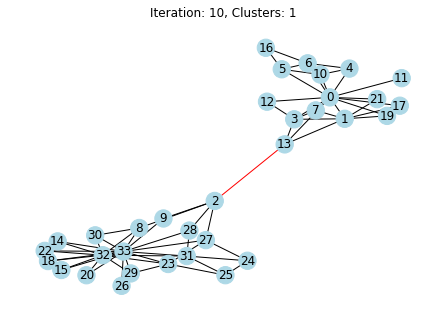
\includegraphics[width=250]{KC_GN10.png}
  \label{fig:GN10}
\end{minipage}%
\begin{minipage}{.5\textwidth}
  \centering
  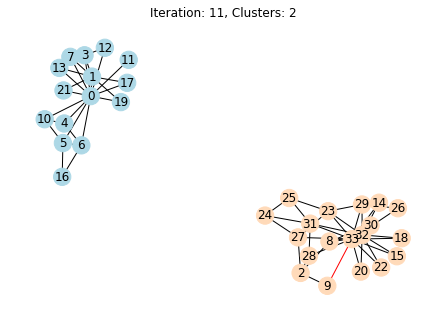
\includegraphics[width=250]{KC_GN11.png}
  \label{fig:GN11}
\end{minipage}
\end{figure}

\clearpage

\noindent\textbf{Q: How many iterations did it take to split the graph?}

It took 11 iterations to split the graph into 2 partitions.

To replicate the Girvan-Newman algorithm, I calculated the betweenness value for all edges and found the edge with the highest value. Then, I drew the graph before removing the edge with the highest betweenness so I could change its color to show which edge was removed for each iteration. I repeated the steps until there were two clusters and the graph was partitioned. The final graph shows the result of the Girvan-Newman algorithm on the Karate Club graph, the 2 partitions showing who went with John vs Mr Hi. To accomplish this, I utilized the Networkx package to calculate edge betweenness and get the connected components.

\begin{lstlisting}[language=Python, caption=Girvan-Newman algorithm function, label=lst:copy]
def girvan_newman(graph):
  # find number of connected components
  partitions = nx.connected_components(graph)
  cluster_count = nx.number_connected_components(graph)
  count = 0

  while(cluster_count == 1):
    # calculate betweenness and find edge with the highest
    edge_betweenness = nx.edge_betweenness_centrality(graph)
    edge_to_remove = max(graph.edges(), key=edge_betweenness.get)
    
    # replace the color in edge_color_list with red if the edge has the maximum betweenness:
    edge_color_list = ["black"]*len(graph.edges)
    for i, edge in enumerate(graph.edges()):
        if edge == edge_to_remove or (edge[1],edge[0]) == edge_to_remove:
            edge_color_list[i] = 'red'

    # find the nodes forming the connected components
    partition_nodes = []
    for node in partitions:
        partition_nodes.append(list(node))

    # create color map to show connected components
    color_map = []
    for node in graph:
        if node in partition_nodes[0]:
            color_map.append('lightblue')
        else: 
            color_map.append('peachpuff') 

    # plot the graph
    plt.figure(count)
    nx.draw(graph, node_color=color_map, edge_color = edge_color_list, with_labels=True)

    # update the number of connected components
    cluster_count = nx.number_connected_components(graph)
    partitions = nx.connected_components(graph)

    # save each graph
    plt.tight_layout()
    plt.title('Iteration: {}, Clusters: {}'.format(count, cluster_count))
    plt.savefig('/content/drive/MyDrive/Colab Notebooks/DATA 440 - Web Science/KC_GN{}.png'.format(count),bbox_inches='tight')

    # remove the edge with the highest betweenness 
    graph.remove_edge(edge_to_remove[0], edge_to_remove[1])

    count+=1
\end{lstlisting}

\section*{3. Compare the actual to the mathematical split}
\noindent \textbf{Compare the connected components of the Girvan-Newman split graph (Q2) with the connected components of the actual split Karate club graph (Q1).}

\noindent\textbf{Q: Did all of the same colored nodes end up in the same group? If not, what is different?}

All of the same colored nodes except for 2 and 8 ended up in the same group. In the actual mathematical split, 2 and 8 were with Mr Hi. While, in the Girvan-Newman graph, 2 and 8 ended up with John.

\section*{References}

\begin{itemize}
    \item{StackOverflow - Saving Matplotlib graph with title} \url{https://stackoverflow.com/questions/64576843/why-when-saving-my-matplotlib-image-the-title-does-not-appear}
    \item{StackOverflow - Coloring spcific edges on a graph} \url{https://stackoverflow.com/questions/34120957/python-networkx-mark-edges-by-coloring-for-graph-drawing}
    \item{Networkx - edge\_betweenness\_centrality} \url{https://networkx.org/documentation/networkx-1.10/reference/generated/networkx.algorithms.centrality.edge_betweenness_centrality.html#networkx.algorithms.centrality.edge_betweenness_centrality}
    \item{Using the Graph data structure in Python} \url{https://www.section.io/engineering-education/graph-data-structure-python/#representing-graphs}
\end{itemize}

\end{document}





